\documentclass[oneside,letterpaper,titlepage]{article}  
\usepackage{makeidx}
\usepackage{graphicx}
\usepackage{natbib} 
\usepackage[reqno]{amsmath}
\usepackage{amssymb}
\usepackage{verbatim}
\usepackage{epsf}
\usepackage{url}
\usepackage{html}
\usepackage{dcolumn}
\usepackage{longtable}
\usepackage{vmargin}
\topmargin=0in

%\setpapersize{USletter}
\newcolumntype{.}{D{.}{.}{-1}}
\newcolumntype{d}[1]{D{.}{.}{#1}}
%\pagestyle{myheadings}
\htmladdtonavigation{
  \htmladdnormallink{%
    \htmladdimg{http://gking.harvard.edu/pics/home.gif}}
  {http://gking.harvard.edu/}}
\newcommand{\hlink}{\htmladdnormallink}

\bodytext{ BACKGROUND="http://gking.harvard.edu/pics/temple.jpg"}
\setcounter{tocdepth}{3}

\newcommand{\VA}{\textsc{VA}}

\title{\VA: Software for Analyzing Verbal Autopsy
  Data\thanks{Available from http://GKing.Harvard.Edu/va via a Creative
    Commons Attribution-Noncommercial-No Derivative Works 3.0, for
    academic use only}}

\author{Gary King\thanks{David Florence Professor of Government, Harvard
    University (Institute for Quantitative Social Science, 1737 Cambridge
    Street, Harvard University, Cambridge MA 02138;
    \texttt{http://GKing.Harvard.Edu}, \texttt{King@Harvard.Edu},
    (617) 495-2027).}  \and %
  Ying Lu\thanks{Assistant Professor, Department of Sociology, University of Colorado at Boulder (3E Ketchum Hall, UCB 327, Boulder, CO 80309.
\texttt{ylu@colorado.edu}, 303-492-7030)}}

% rbuild: replace 'Version ' '\\' Version
\date{Version \\ \today}

%
\makeindex

\begin{document}\maketitle

\begin{rawhtml} 
  <p> [Also available is a down-loadable <a
  href="/va/docs/va.pdf">PDF</a> version of this entire document]
\end{rawhtml}

\tableofcontents
\clearpage

\section{Introduction}


\VA\ implements methods for estimating cause-specific mortality
fractions based on verbal autopsy data introduced in \citet{KinLu08}:
\begin{quote}
  Gary King and Ying Lu.  2008.  ``\hlink{Verbal Autopsy Methods with
    Multiple Causes of Death}{/files/abs/vamc-abs.shtml},''
  \emph{Statistical Science}, Vol. 23, No. 1 (February, 2008): Pp.
  78--91;
  \url{http://GKing.Harvard.Edu//abs/vamc-abs.shtml}.
\end{quote}

The package estimates cause-specific mortality rates in a population
where a set of dichotomous symptoms are available, using the
relationship between symptoms and a multicategory cause-of-death
variable collected from a nearby medical facility.  Estimation is
nonparametric.


\section{Installation}

\VA\ requires \texttt{R} version 2.2.0 or later, available from
\url{http://cran.r-project.org/}.  Installation of \VA\ differs
slightly by operating system.

\subsection{Windows}

Begin the installation process by launching \texttt{R}.  At the
\texttt{R} command prompt, type:
\begin{verbatim}
  > install.packages("VA", repos = "http://gking.harvard.edu", type="source")
\end{verbatim}

\subsection{Linux/Unix}

After starting \texttt{R}, install \VA\ by typing at the \texttt{R}
command prompt:
\begin{verbatim}
  > install.packages("VA", repos = "http://gking.harvard.edu")
\end{verbatim}

You can ignore warning messages.  Alternatively, you may download the
Linux/Unix bundle `\texttt{VA\_XX.tar.gz}', available from
\url{http://gking.harvard.edu/R/CRAN/src/contrib/}, and place it in
your home directory.  Note that `\texttt{XX}' is the current version
number.  Then, at the Linux/Unix command line from your home
directory, type
\begin{verbatim}
  > R CMD INSTALL VA_XX.tar.gz
\end{verbatim}
to install the package.

\section{Examples}

\subsection{Estimating Cause-specific Adult Mortality Fractions}
\label{sec:tanz}

In this section, we give an example of estimating cause-specific
mortality fractions based on simulated data constructed from a verbal
autopsy survey and related hospital deaths. In these verbal autopsy
data, there are 764 registered deaths from hospital and 738 deaths
collected from the general population. The total number of symptoms
are 49, and there are 19 causes of reported deaths. Below we give the
R syntax we use to analyze these data.  The results are plotted in
Figure~\ref{fig1}.

  \begin{verbatim}
  > data(VAdata)
  > FBA<-VAdata[VAdata$region==1,-1]
  > DSS<-VAdata[VAdata$region==2,-1]
  > res1<-va(formula=cbind(S1+...+S49)~cod,
          data=list(FBA,DSS),  nsymp=16,
          n.subset=300,prob.wt=1,
          printit=TRUE,boot.se=FALSE)
  \end{verbatim}

 \begin{figure}[h]
  \centering
  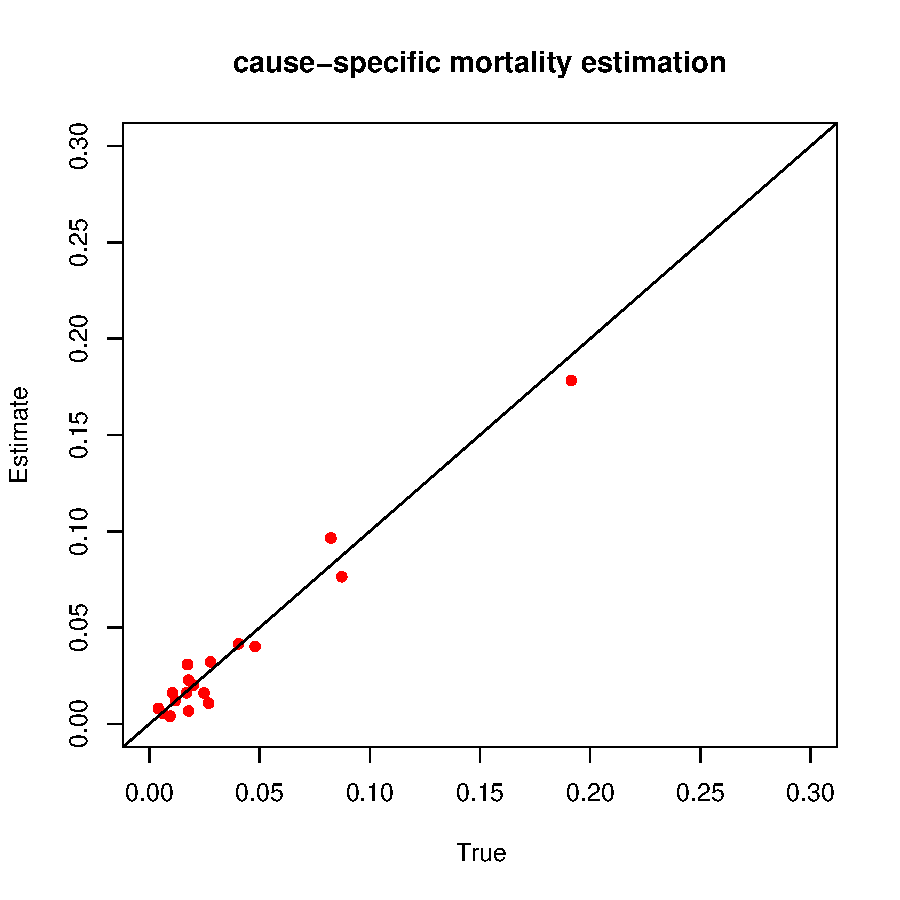
\includegraphics[height=1.9in]{fig1}
  \caption{Estimation of Adult Cause-Specific Mortality Fractions. 
    The observed cause-specific mortality is plotted horizontally and
    our verbal autopsy estimate is plotted vertically.}
  \label{fig1}
\end{figure}

\subsection{Incorporating Additional Information Into Estimation}

Sometimes information about the rate of a specific cause of death is
available from sources other than the verbal autopsy survey.  For
example, the death rate due to homicide and accidents can usually be
determined by direct questioning with little error.  The maternal
death rate is typically lower than a certain known percentage due to
sex and age group restrictions.  In some other situations, a rough
range of the death proportions for specific diseases may be available
from other surveys on health outcomes.  Researchers may also be
willing sometimes to use analyses of neighboring countries or previous
analyses in the same region to put bounds on some of the true
proportions.

Below we give an example of how to incorporate such information into
the \texttt{va} procedure.  In this example, the cause of death
``a13'' and ``a18'' are fixed at 21.6\% and 8\%, and the fraction of
cause ``a14'' is expected to be estimated between 0.5\% and 1\%.
\begin{verbatim}
 res2 <- va(formula=cbind(S1+...+S49)~cod, 
            fix=c("a13=0.216", "a18=0.08"),
            bound=c("0.005<a14<0.01"),
            data=list(FBA,DSS),  nsymp=16,
            n.subset=10,prob.wt=1,printit=TRUE,boot.se=FALSE)
\end{verbatim}



\section{\texttt{R} Function Reference}

\subsection{Function \texttt{va()}}

This function estimates the cause-specific mortality fractions from
verbal autopsy data and hospital gold-standard cause-of-death
diagnostics.  It can also compute the bootstrap-based standard errors
of the cause-specific mortality fractions.

\subsubsection{Usage}

\begin{verbatim}
     va(formula, data=list(hospital, community), nsymp=16, n.subset=300,
method=``quadOpt'', fix=NA, bound=NA, 
prob.wt=1, boot.se=FALSE, nboot=300, printit=TRUE, print.reg.size=FALSE)
\end{verbatim}

\subsubsection{Inputs}

\begin{description}
\item[formula] A formula object. The left side of the formula is the
  collection of symptoms. The right side is the cause of death.  For
  example, if there are totally 5 symptoms, named
  \texttt{fever},\texttt{coughing},\texttt{chestpain},\texttt{dizziness},
  \texttt{shortbreath}, and the cause of death variable is
  \texttt{death}, then the formula can be written as:

    \begin{verbatim}
       formula=cbind(fever, coughing, chestpain, dizziness, shortbreath)~death
    \end{verbatim}
  or for short:
    \begin{verbatim}
       formula=cbind(fever, ... ,shortbreath)~death
       \end{verbatim}
  Note that the short way of writing formula requires the symptoms
  variables are located in a consecutive block in the data starting
  from \texttt{fever} and ending with \texttt{shortbreath}.
Note that the current version requires the variable on the right hand
   side of the formula, \texttt{death} in this example, to be present in
   the \texttt{community} sample. If it is unknown in the
   \texttt{community} sample, the user needs to create such variable
   with arbitrary numerical values.
\item[data] A list of two datasets. The first is the hospital data,
  which contains a known cause of death for each individual, and a
  collection of symptoms from verbal autopsy studies.  The second is
  the community data where typically only the symptoms are available
  from the verbal autopsy study. The known cause of death diagnostics
  may also be known in the community data if this is a validation
  study, but will not be used during estimation.  Variable names must
  be exactly the same in two data sets.
\item[nsymp] A positive integer specifying the number of symptoms to
  be subset from all symptoms for estimating cause specific mortality
  fractions at each iteration. For the choice of \texttt{nsymp}, refer   
  to King and Lu (2006). For practical purpose, we give the following 
  recommendations: for total number of causes of death \texttt{D<=10}, 
  use 7-12 symptoms; for \texttt{D>10}, use 12-18 symptoms. If the 
  number of observations is large in both hospital and community samples,
  for example, over 1000 cases total, use more symptoms, 
  otherwise use fewer. Sensitivity analysis can also 
  be used to choose \texttt{nsymp}. In general, the results stabilize in 
  the right range of the choices of \texttt{nsymp}. Default=16.
\item[n.subset] A positive integer specifying the total number of
  draws of different subsets of symptoms.  Default=300.
\item[method] A string specifying the computational procedure
 used to estimate the cause specific mortality fractions. When 
\texttt{method=''quadOpt''}, CSMF is estimated via constrained 
quadratic programming. A subroutine (\texttt{Solve.QP}) from the 
\texttt{quadprog} package is called to perform the constrained 
quadratic optimization task. When \texttt{method=``constrainLS''},
CSMF is estimated via constrained least squares. The default method
is \texttt{quadprog} as it is faster and more stable. 
\item[fix] A vector of strings that allow the user to fix a subset of
  the cause-specific mortality fractions to predetermined values
  chosen by the user (based on, e.g., the information obtained from
  other sources or prior knowledge).  For example, setting
  \texttt{fix=c("malaria=0.15", "injuries=0.05")} fixes the mortality
  fractions due to malaria and injuries to 15\% and 5\%, respectively.
  Running \texttt{va} in this case will then attempt to allocate only the
  remaining 80\% of the deaths.  The default is \texttt{NA}, which
  means no constraint is imposed.
\item[bound] A vector of strings that allow the user to set fixed
  lower and upper bounds for a given subset of the cause specific
  mortality fractions (based on, e.g., information obtained from other
  sources or prior knowledge).  For example, running \texttt{va} while setting
  \texttt{bound=c("0.2 < HIV < 0.35", "0.1 < TB < 0.15")} restricts
  the mortality fraction due to HIV to be between 20\% and 35\% and the
  TB rate is constrained to be between 10\% and 15\%.  Causes not
  specified here are assumed to be bounded only by 0 and 1, and with
  the collection still constrained to the simplex.  The default is
  \texttt{NA}, which means no constraint is imposed.
\item[prob.wt] A positive integer or a vector of weights that 
  determines how likely a symptom is being selected in a subset. 
  When \texttt{prob.wt} is a user input vector, it needs to be a vector 
  of probabilities and sum up to 1. The length of \texttt{prob.wt} 
  needs to be equal to the total number of symptoms. 
  When \texttt{prob.wt=1}, binomial weights which are proportion to 
  the inverse of variances of the each reported binary symptom variable.   
  When \texttt{prob.wt=0}, all symptoms will be equally selected. 
  Default=1.
\item[boot.se] A Logical value. If \texttt{TRUE}, bootstrap standard
  errors of the CSMF are estimated.  This option typically takes a lot
  of computing time. The default is \texttt{FALSE}.
\item[nboot] A positive integer. If \texttt{boot.se=TRUE}, it
  specifies the number of bootstrapping samples taken to estimate the
  standard errors of CSMF. The default is \texttt{300}.
\item[printit] Logical value. If \texttt{TRUE}, the progress of the
  estimation procedure is printed on the screen.
 \item[clean.data] Logical value. If \texttt{TRUE}, \texttt{va}
    automatically deletes the symptoms variables(left-hand side of the
    formula) where there is no variation (all 0s or 1s). If
    \texttt{FALSE}, the user must make sure the data is cleaned before
    hand(which is recommended). 
  \item[print.reg.size] Logical value. If \texttt{TRUE}, the size of the
  regression matrix is printed at each step of sub-sampling. It provides
  helpful information for user to choose the number of symptoms to
  subsample. It is recommended to print the size of the regression
  matrix for different values of \texttt{nsymp} with a small size of
  \texttt{n.subset}. 
\end{description}

\subsubsection{Value}

An object of class ``VA'', a list containing the following elements:
\begin{description}
\item[est.CSMF] The estimated cause-specific mortality fractions.
\item[true.CSMF] The observed cause-specific mortality fractions,
  whenever available.
\item[est.se] The bootstrap standard errors of \texttt{est.CSMF} when
  \texttt{boot.se=TRUE}.
\item[true.CSMF.bootmean] The bootstrap mean of the observed
  cause-specific mortality fractions when they are available and when
  \texttt{boot.se=TRUE}.
\item[true.bootse] The bootstrap standard errors of the observed
  cause-specific mortality fractions when they are available and when
  \texttt{boot.se=TRUE}.
 \end{description}


\subsection{Function \texttt{va.gcv()}}
This function use the method of general cross-validation to find the best 
\texttt{nsymp}, the number of symtoms to be subset from all symptoms for 
estimating the cause specific mortality fractions. 

\subsubsection{Usage}

\begin{verbatim}
va.gcv(formula, data=list(hospital, community), nsymp.vec, 
       n.subset=300, prob.wt=1, boot.se=FALSE, nboot=1, 
       printit=FALSE, print.reg.size=TRUE)
\end{verbatim}

\subsubsection{Inputs}

\begin{description}
\item[formula] A formula object. The left side of the formula is the
  collection of symptoms. The right side is the cause of death.  For
  example, if there are totally 5 symptoms, named
  \texttt{fever},\texttt{coughing},\texttt{chestpain},\texttt{dizziness},
  \texttt{shortbreath}, and the cause of death variable is
  \texttt{death}, then the formula can be written as:

    \begin{verbatim}
       formula=cbind(fever, coughing, chestpain, dizziness, shortbreath)~death
    \end{verbatim}
  or for short:
    \begin{verbatim}
       formula=cbind(fever, ... ,shortbreath)~death
       \end{verbatim}
  Note that the short way of writing formula requires the symptoms
  variables are located in a consecutive block in the data starting
  from \texttt{fever} and ending with \texttt{shortbreath}.
Note that the current version requires the variable on the right hand
   side of the formula, \texttt{death} in this example, to be present in
   the \texttt{community} sample. If it is unknown in the
   \texttt{community} sample, the user needs to create such variable
   with arbitrary numerical values.
\item[data] A list of two datasets. The first is the hospital data,
  which contains a known cause of death for each individual, and a
  collection of symptoms from verbal autopsy studies.  The second is
  the community data where typically only the symptoms are available
  from the verbal autopsy study. The known cause of death diagnostics
  may also be known in the community data if this is a validation
  study, but will not be used during estimation.  Variable names must
  be exactly the same in two data sets.
\item[nsymp.vec] A vector of positive integer, containing different
  \texttt{nsymp} that can be used by \texttt{va()}.  For a total of
  \texttt{J} number of causes of death and a total of \texttt{ns} symptoms
  in the sample, \texttt{nsymp.vec} cna be set to be a vector
  \texttt{a:b}, while \texttt{a} is the smallest integer than $2^a>J$.
  \texttt{b} is typically set to be \texttt{floor{0.75*b}}. If sample
  size is small, \texttt{b} can be set to smaller value to avoid
  function exiting due to data sparsity.  No default value is set.
  \item[n.subset] A positive integer specifing the total number of
     subsets and thus estimations of all symptoms.
     The default is \texttt{300}.
   \item[prob.wt] A positive integer or a vector of weights that determines how
     likely a symptom is of being selected for a subset. When
     \texttt{prob.wt} is a user input vector, it needs to be a vector 
     of probabilities and sum up to 1. The length of
     \texttt{[prob.wt} needs to be equal to the total number of symptoms.
     When \texttt{prob.wt=1}, binomial weights which are proportion to 
     the inverse of variances of the each reported binary symptom variable.   
     When \texttt{prob.wt=0}, all symptoms will be equally selected. 
     The default is \texttt{1}.
   \item[boot.se] A Logical value. If \texttt{TRUE}, bootstrap
     standard errors of the CSMF are estimated.  This typically takes a lot
     of computing time. It is highly suggested to set
     \texttt{boot.se=FALSE} in \texttt{va.gcv}. Default=\texttt{FALSE}.
  \item[nboot] A positive integer. If \texttt{boot.se=TRUE}, it
    specifies the number of bootstrapping samples taken to estimate the
    standard errors of CSMF. The default is \texttt{1}.
  \item[printit] Logical value. If \texttt{TRUE}, the progress of the
    estimation procedure will be printed on the screen.
  \item[print.reg.size] Logical value. If \texttt{TRUE}, the size of the
  regression matrix is printed at each step of subsampling. It provides
  helpful information for user to choose the number of symptoms to
  subsample. It is recommended to print the size of the regression
  matrix for different values of \texttt{nsymp} with a small size of
  \texttt{n.subset}. 
\end{description}

\subsubsection{Value}
An object of class ``VA'', a list containing the following elements:
\begin{description}
 \item[best.symp] It returns the \texttt{nsymp}, the size of
  subset that minimizes mean square error between estimated
  cause-specific mortality fraction and the observed cause-specific
  mortality fraction. 
\item[mse] It is a vector of  mean square errors
  associated with each size of the subsets (as specified in \texttt{symp.vec}).
\end{description}

\bibliographystyle{apsr} 
\bibsep=0in 
\bibliography{gk.bib,gkpubs.bib}
\end{document}


